\section{Comunicação}
Conforme explicado anteriormente, neste projeto utilizamos tanto protocolos de comunicação próprios quanto os elaborados comercialmente. A arquitetura desenvolvida aqui busca viabilizar a robustez do sistema, trabalhando em um nível local e outro nível remoto, onde o usuário terá o controle de sua casa por meio do Smartphone ou computador pessoal.

Teremos um serviço de nuvem (que será descrito na seção de software) que receberá as requisições do usuário, por meio de um cliente web ou nativo. Esse servidor processará as requisições, aplicando os filtros de segurança necessário, de modo a consultar a autenticidade do pedido, e se aquele usuário possui as permissões necessárias para o serviço que deseja operar. Os serviços da nuvem se comunicarão com o servidor local, da casa requisitada, o qual também aplicará os filtros de segurança necessários, e realizará a comunicação com os atuadores.

A infraestrutura de comunicação entre a nuvem e o servidor local, e o servidor local e os sensores e atuadores utilizará o protocolo de aplicação \wmqtt{}, referência em aplicações IoT no mundo. O protocolo \wmqtt{} é estabelecido em cima dos protocolos TCP/IP (nas camadas inferiores) e é orientado é orientado à sessão, diferentemente do protocolo HTTP, de mesma camada.

O protocolo \wmqtt{} é do tipo Pub/Sub (de \textit{publisher/subscriber}) e é estritamente orientado à tópicos. Assim, um subscriber deve se inscrever a um tópico de seu interesse, e receberá todas as publicações que um publisher realizar. Os tópicos são organizados com estrutura semelhante a de um sistema de arquivos Unix, com níveis hierárquicos, separados por barras, de modo que o subscriber pode se inscrever para tópicos utilizando wildcards (* e +, os quais são válidos para mais de um nível e um único nível, respectivamente).

Para interconectar os tópicos, com publishers e subscribers, é necessário um agente que realiza a transmissão das mensagens, e que garante a segurança e confiabilidade. Esse agente é conhecido como Broker (em versões anteriores) ou Server (na versão atual, V3.1.1). O broker irá permitir ou negar a subscrição a determinado tópico, ou a publicação.

A segurança da troca de mensagens é realizada por meio do protocolo TLS (\textit{Transport Layer Security}) que encripta os segmentos na camada de transporte. Toda a parte de segurança e criptografia será detalhada no momento oportuno, bem como a organização dos tópicos implementados.

Além disso, o protocolo \wmqtt{} oferece três tipos de QoS (\textit{Quality of Service}), possibilitando: diminuir o overhead ao máximo, enviando a mensagem uma única vez, na configuração mais simples; garantir que a mensagem seja entregue no mínimo uma vez, na configuração de segundo nível; garantir que a mensagem seja entregue exatamente uma vez, no terceiro nível, o que aumenta o overhead, consequentemente.

As mensagens são transmitidas em texto puro, e é necessário estabelecer um protocolo para a sua utilização. Utilizaremos aqui o protocolo que define a configurações das mensagens, desenvolvido no projeto HomeSky.

O broker Mosquitto será utilizado, e foi escolhido por ser amplamente adotado em projetos de IoT, além de ser open source e com licença abrangente (MIT). Entretanto, há diversas possibilidades, como o HiveMQ, adotado no projeto HomeSky, e com grande uso em aplicações enterprise.

A arquitetura de comunicação é representada pelo diagrama abaixo, com um alto nível de abstração, cujos detalhes serão vistos no momento oportuno, com granularidade menor.

% TODO o diagrama ta diferente no arquivo da quarta entrega
% TODO update: Provavelmente esta certo agora, mas precisamos confirmar

\begin{figure}[H]
	\centering
	\caption{}
  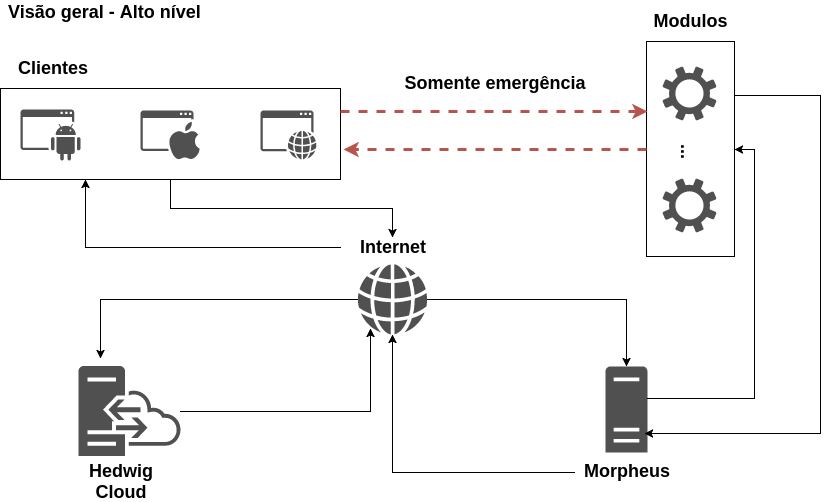
\includegraphics[width=0.8\textwidth]{arquiteturaHedwig}
\label{fig:diagramaComunicacao}
\end{figure}

\subsection{Entre módulos e controlador local}
\subsection{Entre controlador local e nuvem}
\subsection{Entre cliente web e nuvem}
\subsection{Entre app backup e módulos}
